\documentclass[twoside]{book}

% Packages required by doxygen
\usepackage{fixltx2e}
\usepackage{calc}
\usepackage{doxygen}
\usepackage[export]{adjustbox} % also loads graphicx
\usepackage{graphicx}
\usepackage[utf8]{inputenc}
\usepackage{makeidx}
\usepackage{multicol}
\usepackage{multirow}
\PassOptionsToPackage{warn}{textcomp}
\usepackage{textcomp}
\usepackage[nointegrals]{wasysym}
\usepackage[table]{xcolor}

% Font selection
\usepackage[T1]{fontenc}
\usepackage[scaled=.90]{helvet}
\usepackage{courier}
\usepackage{amssymb}
\usepackage{sectsty}
\renewcommand{\familydefault}{\sfdefault}
\allsectionsfont{%
  \fontseries{bc}\selectfont%
  \color{darkgray}%
}
\renewcommand{\DoxyLabelFont}{%
  \fontseries{bc}\selectfont%
  \color{darkgray}%
}
\newcommand{\+}{\discretionary{\mbox{\scriptsize$\hookleftarrow$}}{}{}}

% Page & text layout
\usepackage{geometry}
\geometry{%
  a4paper,%
  top=2.5cm,%
  bottom=2.5cm,%
  left=2.5cm,%
  right=2.5cm%
}
\tolerance=750
\hfuzz=15pt
\hbadness=750
\setlength{\emergencystretch}{15pt}
\setlength{\parindent}{0cm}
\setlength{\parskip}{3ex plus 2ex minus 2ex}
\makeatletter
\renewcommand{\paragraph}{%
  \@startsection{paragraph}{4}{0ex}{-1.0ex}{1.0ex}{%
    \normalfont\normalsize\bfseries\SS@parafont%
  }%
}
\renewcommand{\subparagraph}{%
  \@startsection{subparagraph}{5}{0ex}{-1.0ex}{1.0ex}{%
    \normalfont\normalsize\bfseries\SS@subparafont%
  }%
}
\makeatother

% Headers & footers
\usepackage{fancyhdr}
\pagestyle{fancyplain}
\fancyhead[LE]{\fancyplain{}{\bfseries\thepage}}
\fancyhead[CE]{\fancyplain{}{}}
\fancyhead[RE]{\fancyplain{}{\bfseries\leftmark}}
\fancyhead[LO]{\fancyplain{}{\bfseries\rightmark}}
\fancyhead[CO]{\fancyplain{}{}}
\fancyhead[RO]{\fancyplain{}{\bfseries\thepage}}
\fancyfoot[LE]{\fancyplain{}{}}
\fancyfoot[CE]{\fancyplain{}{}}
\fancyfoot[RE]{\fancyplain{}{\bfseries\scriptsize Generated by Doxygen }}
\fancyfoot[LO]{\fancyplain{}{\bfseries\scriptsize Generated by Doxygen }}
\fancyfoot[CO]{\fancyplain{}{}}
\fancyfoot[RO]{\fancyplain{}{}}
\renewcommand{\footrulewidth}{0.4pt}
\renewcommand{\chaptermark}[1]{%
  \markboth{#1}{}%
}
\renewcommand{\sectionmark}[1]{%
  \markright{\thesection\ #1}%
}

% Indices & bibliography
\usepackage{natbib}
\usepackage[titles]{tocloft}
\setcounter{tocdepth}{3}
\setcounter{secnumdepth}{5}
\makeindex

% Hyperlinks (required, but should be loaded last)
\usepackage{ifpdf}
\ifpdf
  \usepackage[pdftex,pagebackref=true]{hyperref}
\else
  \usepackage[ps2pdf,pagebackref=true]{hyperref}
\fi
\hypersetup{%
  colorlinks=true,%
  linkcolor=blue,%
  citecolor=blue,%
  unicode%
}

% Custom commands
\newcommand{\clearemptydoublepage}{%
  \newpage{\pagestyle{empty}\cleardoublepage}%
}

\usepackage{caption}
\captionsetup{labelsep=space,justification=centering,font={bf},singlelinecheck=off,skip=4pt,position=top}

%===== C O N T E N T S =====

\begin{document}

% Titlepage & ToC
\hypersetup{pageanchor=false,
             bookmarksnumbered=true,
             pdfencoding=unicode
            }
\pagenumbering{alph}
\begin{titlepage}
\vspace*{7cm}
\begin{center}%
{\Large R\+OS lib, camera stream node }\\
\vspace*{1cm}
{\large Generated by Doxygen 1.8.13}\\
\end{center}
\end{titlepage}
\clearemptydoublepage
\pagenumbering{roman}
\tableofcontents
\clearemptydoublepage
\pagenumbering{arabic}
\hypersetup{pageanchor=true}

%--- Begin generated contents ---
\chapter{R\+OS library for image transmission.}
\label{index}\hypertarget{index}{}This template for a R\+OS library was intended to be implemented in the Rescue Robot design by us for Tec de Monterrey, Campus Guadalajara.~\newline
The same library contain both nodes (transmit and recevie), but it is not necessary to include the receive node in the robot (this could avoid unnecessary use of memory).\begin{DoxyAuthor}{Authors}
Humberto Regla González~\newline
Antonio Emmanuel García Vázquez~\newline
Moisés Alejandro García Pérez
\end{DoxyAuthor}
\hypertarget{index_use}{}\section{Use and explore the library}\label{index_use}
Here you could find the information regarding the code. All the code related documentation can be found under each code file and these files can be found under the \char`\"{}\+Files\char`\"{} section above. You can also find a page, under the \char`\"{}\+Related Pages\char`\"{} section above, called \char`\"{}\+R\+O\+S intro\char`\"{}; in this page you can find a very brief introduction to how to install and use R\+OS.\hypertarget{index_contact}{}\section{Contact info}\label{index_contact}
Students from Tec de Monterrey Campus Guadalajara can get in contact with us for future references and support. This apply for any components of the robot.~\newline
We understand the complexity of the system is in the mechanic section.~\newline
You can try to get our phone numbers from Oscar Carbajal, but here I put our personal emails for contact purposes\+:~\newline
Antonio Garcia (mechanics chief)\+: \href{mailto:tony.garcia.vz@gmail.com}{\tt tony.\+garcia.\+vz@gmail.\+com} / aegv.\+com.\+mx~\newline
Humberto Regla (software, mechanics)\+: \href{mailto:htoregla1@hotmail.com}{\tt htoregla1@hotmail.\+com}~\newline
Moisés García (mechanics)\+: \href{mailto:magp.imt@gmail.com}{\tt magp.\+imt@gmail.\+com} 
\chapter{R\+OS intro}
\label{ros}
\Hypertarget{ros}
R\+OS Melodic installation for Ubuntu 18\+:~\newline
\href{http://wiki.ros.org/melodic/Installation/Ubuntu}{\tt http\+://wiki.\+ros.\+org/melodic/\+Installation/\+Ubuntu} \begin{DoxyVerb}                          CREATE ENVIRONMENT
\end{DoxyVerb}


It is important to first create a folder to put the R\+OS environment in it.

You could add the default environment variables with\+:~\newline
{\ttfamily source /opt/ros/kinetic/setup.bash}

Depending on version you need, instead of the above\+:~\newline
{\ttfamily source /opt/ros/melodic/setup.bash}

{\bfseries Y\+OU DO N\+OT A\+L\+W\+A\+YS H\+A\+VE TO S\+O\+U\+R\+CE T\+HE D\+E\+F\+A\+U\+LT V\+A\+R\+I\+A\+B\+L\+ES, B\+UT IT IS C\+O\+N\+V\+E\+N\+I\+E\+NT}.

Create the workspace creating the two main directories (must place the terminal in desired folder first)\+:~\newline
{\ttfamily mkdir -\/p $<$environment\+\_\+folder\+\_\+name$>$/src}

Initialize the environment with\+:~\newline
{\ttfamily cd $<$environment\+\_\+folder\+\_\+name$>$~\newline
catkin\+\_\+make}

Overlay catkin workspace with\+:~\newline
{\ttfamily source devel/setup.\+bash}

Finally, you can check your workspace with\+:~\newline
{\ttfamily echo \$\+R\+O\+S\+\_\+\+P\+A\+C\+K\+A\+G\+E\+\_\+\+P\+A\+TH} \begin{DoxyVerb}                            USEFUL COMMANDS
\end{DoxyVerb}


Start a master in a separate terminalwith\+:~\newline
{\ttfamily roscore}

To be able to run a node from a created package you must add it as source.~\newline
To do this you must go to the environment folder and run\+:~\newline
{\ttfamily catkin\+\_\+make}

This will run all of your packages and add them to this environment.~\newline
Now, add the environment with\+:~\newline
{\ttfamily source devel/setup.\+bash}

Once you did this, you can use rosrun to run your node.

Run a node with\+:~\newline
{\ttfamily rosrun $<$package\+\_\+name$>$ $<$node\+\_\+name$>$}

Check active nodes with\+:~\newline
{\ttfamily rosnode list}

Retrieve information about a node with\+:~\newline
{\ttfamily rosnode info $<$node\+\_\+name$>$}

List active topics with\+:~\newline
{\ttfamily rostopic list}

Subscribe and print the contents of a topic with\+:~\newline
{\ttfamily rostopic echo /topic}

Show information about a topic with\+:~\newline
{\ttfamily rostopic info /topic} \begin{DoxyVerb}                           CREATE A PACKAGE
\end{DoxyVerb}


Once you created the environment, locate a terminal in the src folder and run\+:~\newline
{\ttfamily catkin\+\_\+create\+\_\+pkg $<$package\+\_\+name$>$ \{$<$dependencies$>$\}}

{\bfseries N\+O\+TE\+:} {\itshape D\+E\+P\+E\+N\+D\+E\+N\+C\+I\+ES A\+RE O\+T\+H\+ER P\+A\+C\+K\+A\+G\+ES N\+E\+E\+D\+ED BY T\+HE F\+I\+R\+ST P\+A\+C\+K\+A\+GE.}

Once you run the command you will have to modify the package.\+xml file.~\newline
Important thing to modify are\+:~\newline
\begin{DoxyItemize}
\item Package name\+: Name of the package. Defined at creation. \item Version number\+: Version of the developed project. \item Authors\+: Project contributors. \item Dependencies on other packages\+: Very important. Some options appear commented. Check for necessary ones.\end{DoxyItemize}
You will also have to modify the C\+Make\+Lists.\+txt, taking care of at least\+:~\newline
\begin{DoxyItemize}
\item {\ttfamily cmake\+\_\+minimum\+\_\+required(V\+E\+R\+S\+I\+ON 2.\+8.\+3)} \+: Version \item {\ttfamily project($<$package\+\_\+name$>$)} \+: Package name \item {\ttfamily add\+\_\+definitions(--std=c++11)} \+: C++11 by default \item {\ttfamily find\+\_\+package(catkin R\+E\+Q\+U\+I\+R\+ED} \+: Required packages \item {\ttfamily C\+O\+M\+P\+O\+N\+E\+N\+TS $<$package1$>$ $<$package2$>$ )} \item {\ttfamily catkin\+\_\+package (} \+: Starting from here, required files are included~\newline
 {\ttfamily I\+N\+C\+L\+U\+D\+E\+\_\+\+D\+I\+RS $<$directory\+\_\+with\+\_\+include\+\_\+files$>$} \+: Directory with headers~\newline
 {\ttfamily \# L\+I\+B\+R\+A\+R\+I\+ES} \+: Libraries in the project~\newline
 {\ttfamily C\+A\+T\+K\+I\+N\+\_\+\+D\+E\+P\+E\+N\+DS $<$library\+\_\+\+A$>$ $<$library\+\_\+\+B$>$} \+: Required libraries~\newline
 {\ttfamily \# D\+E\+P\+E\+N\+DS )} \+: Package dependent projects~\newline
\item {\ttfamily include\+\_\+directories(include \$\{catkin\+\_\+\+I\+N\+C\+L\+U\+D\+E\+\_\+\+D\+I\+RS\})} \item {\ttfamily add\+\_\+executable(\$\{P\+R\+O\+J\+E\+C\+T\+\_\+\+N\+A\+ME\}} \+: Declare a C++ executable name \item {\ttfamily src/\$\{P\+R\+O\+J\+E\+C\+T\+\_\+\+N\+A\+ME\}\+\_\+node.\+cpp} \+: Declare all source files \item {\ttfamily src/comm\+\_\+interface.\+cpp )} \item {\ttfamily target\+\_\+link\+\_\+libraries(\$\{P\+R\+O\+J\+E\+C\+T\+\_\+\+N\+A\+ME\}} \+: Specify the libraries to link the executable against \item {\ttfamily \$\{catkin\+\_\+\+L\+I\+B\+R\+A\+R\+I\+ES\})}\end{DoxyItemize}
The main components of a C\+Make\+Lists.\+txt are\+:~\newline
\begin{DoxyItemize}
\item Required C\+Make Version~\newline
 {\ttfamily cmake\+\_\+minimum\+\_\+required()} \item Package Name\+:~\newline
 {\ttfamily project($<$package\+\_\+name$>$)} \item Find other C\+Make/\+Catkin packages needed for build\+:~\newline
 {\ttfamily find package($<$dependencies$>$)} \item Message/\+Service/\+Action Generators\+:~\newline
 {\ttfamily add message files()~\newline
 add service files()~\newline
 add action files()} \item Invoke message/service/action generation\+:~\newline
 {\ttfamily generate messages()} \item Specify package build info export\+:~\newline
 {\ttfamily catkin package()} \item Libraries/\+Executable to build\+:~\newline
 {\ttfamily add library()~\newline
 add executable()~\newline
 target link libraries()} \item Tests to build\+:~\newline
 {\ttfamily catkin add gtest()} \item Install rules~\newline
 {\ttfamily install()} \end{DoxyItemize}

\chapter{File Index}
\section{File List}
Here is a list of all documented files with brief descriptions\+:\begin{DoxyCompactList}
\item\contentsline{section}{/home/hrg/\+Documents/\+R\+O\+S/ros\+\_\+ws/src/ros\+\_\+camera\+\_\+lib/include/img\+\_\+listen/api/\hyperlink{img__listen__api_8hpp}{img\+\_\+listen\+\_\+api.\+hpp} }{\pageref{img__listen__api_8hpp}}{}
\item\contentsline{section}{/home/hrg/\+Documents/\+R\+O\+S/ros\+\_\+ws/src/ros\+\_\+camera\+\_\+lib/include/img\+\_\+listen/app/\hyperlink{img__listen_8hpp}{img\+\_\+listen.\+hpp} }{\pageref{img__listen_8hpp}}{}
\item\contentsline{section}{/home/hrg/\+Documents/\+R\+O\+S/ros\+\_\+ws/src/ros\+\_\+camera\+\_\+lib/include/img\+\_\+listen/hal/\hyperlink{img__listen__hal_8hpp}{img\+\_\+listen\+\_\+hal.\+hpp} }{\pageref{img__listen__hal_8hpp}}{}
\item\contentsline{section}{/home/hrg/\+Documents/\+R\+O\+S/ros\+\_\+ws/src/ros\+\_\+camera\+\_\+lib/src/img\+\_\+listen/api/\hyperlink{img__listen__api_8cpp}{img\+\_\+listen\+\_\+api.\+cpp} }{\pageref{img__listen__api_8cpp}}{}
\item\contentsline{section}{/home/hrg/\+Documents/\+R\+O\+S/ros\+\_\+ws/src/ros\+\_\+camera\+\_\+lib/src/img\+\_\+listen/app/\hyperlink{img__listen_8cpp}{img\+\_\+listen.\+cpp} }{\pageref{img__listen_8cpp}}{}
\item\contentsline{section}{/home/hrg/\+Documents/\+R\+O\+S/ros\+\_\+ws/src/ros\+\_\+camera\+\_\+lib/src/img\+\_\+listen/hal/\hyperlink{img__listen__hal_8cpp}{img\+\_\+listen\+\_\+hal.\+cpp} }{\pageref{img__listen__hal_8cpp}}{}
\end{DoxyCompactList}

\chapter{File Documentation}
\hypertarget{cam__stream__api_8hpp}{}\section{/home/hrg/\+Documents/\+R\+O\+S/ros\+\_\+ws/src/ros\+\_\+camera\+\_\+lib/include/cam\+\_\+stream/api/cam\+\_\+stream\+\_\+api.hpp File Reference}
\label{cam__stream__api_8hpp}\index{/home/hrg/\+Documents/\+R\+O\+S/ros\+\_\+ws/src/ros\+\_\+camera\+\_\+lib/include/cam\+\_\+stream/api/cam\+\_\+stream\+\_\+api.\+hpp@{/home/hrg/\+Documents/\+R\+O\+S/ros\+\_\+ws/src/ros\+\_\+camera\+\_\+lib/include/cam\+\_\+stream/api/cam\+\_\+stream\+\_\+api.\+hpp}}
{\ttfamily \#include $<$string$>$}\newline
Include dependency graph for cam\+\_\+stream\+\_\+api.\+hpp\+:\nopagebreak
\begin{figure}[H]
\begin{center}
\leavevmode
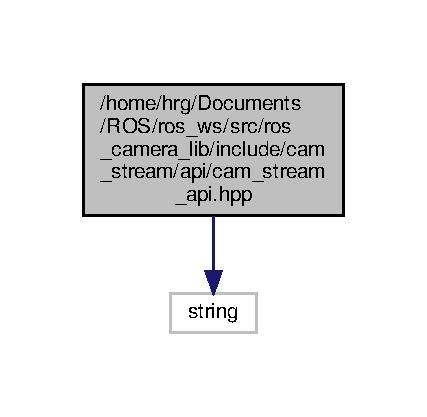
\includegraphics[width=205pt]{cam__stream__api_8hpp__incl}
\end{center}
\end{figure}
This graph shows which files directly or indirectly include this file\+:\nopagebreak
\begin{figure}[H]
\begin{center}
\leavevmode
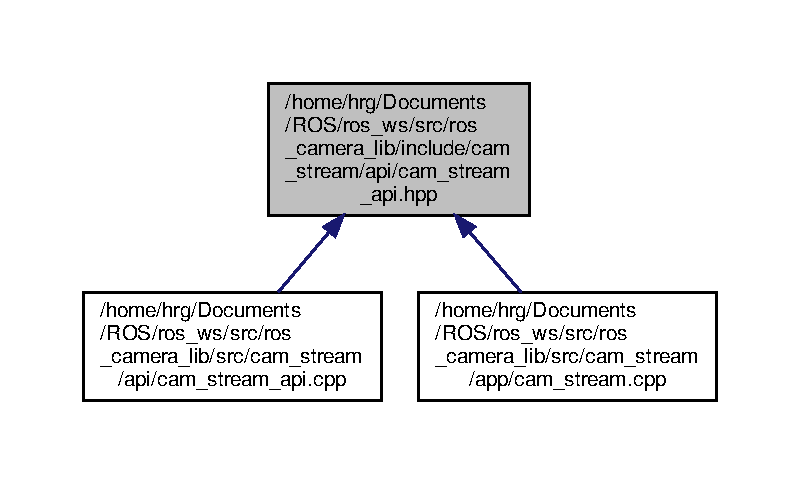
\includegraphics[width=350pt]{cam__stream__api_8hpp__dep__incl}
\end{center}
\end{figure}
\subsection*{Functions}
\begin{DoxyCompactItemize}
\item 
void \hyperlink{cam__stream__api_8hpp_a071b3460290577ea5f2dde4bbceb43a3}{system\+\_\+init} (int argc, char $\ast$$\ast$argv, std\+::string node\+\_\+name, int video\+\_\+source)
\item 
int \hyperlink{cam__stream__api_8hpp_a77353b4935e897316414f01ccd30b117}{system\+\_\+ok} (void)
\item 
void \hyperlink{cam__stream__api_8hpp_aa1f1f7d9c7b32ebc5ee26f4d9748d99f}{stream} (void)
\item 
void \hyperlink{cam__stream__api_8hpp_ac6d72bbe9a798feae197f4c8ce164b08}{finish\+\_\+system} (void)
\end{DoxyCompactItemize}


\subsection{Function Documentation}
\mbox{\Hypertarget{cam__stream__api_8hpp_ac6d72bbe9a798feae197f4c8ce164b08}\label{cam__stream__api_8hpp_ac6d72bbe9a798feae197f4c8ce164b08}} 
\index{cam\+\_\+stream\+\_\+api.\+hpp@{cam\+\_\+stream\+\_\+api.\+hpp}!finish\+\_\+system@{finish\+\_\+system}}
\index{finish\+\_\+system@{finish\+\_\+system}!cam\+\_\+stream\+\_\+api.\+hpp@{cam\+\_\+stream\+\_\+api.\+hpp}}
\subsubsection{\texorpdfstring{finish\+\_\+system()}{finish\_system()}}
{\footnotesize\ttfamily void finish\+\_\+system (\begin{DoxyParamCaption}\item[{void}]{ }\end{DoxyParamCaption})}

Function in charge of releasing the system resources. \mbox{\Hypertarget{cam__stream__api_8hpp_aa1f1f7d9c7b32ebc5ee26f4d9748d99f}\label{cam__stream__api_8hpp_aa1f1f7d9c7b32ebc5ee26f4d9748d99f}} 
\index{cam\+\_\+stream\+\_\+api.\+hpp@{cam\+\_\+stream\+\_\+api.\+hpp}!stream@{stream}}
\index{stream@{stream}!cam\+\_\+stream\+\_\+api.\+hpp@{cam\+\_\+stream\+\_\+api.\+hpp}}
\subsubsection{\texorpdfstring{stream()}{stream()}}
{\footnotesize\ttfamily void stream (\begin{DoxyParamCaption}\item[{void}]{ }\end{DoxyParamCaption})}

Function in charge of streaming the image. \mbox{\Hypertarget{cam__stream__api_8hpp_a071b3460290577ea5f2dde4bbceb43a3}\label{cam__stream__api_8hpp_a071b3460290577ea5f2dde4bbceb43a3}} 
\index{cam\+\_\+stream\+\_\+api.\+hpp@{cam\+\_\+stream\+\_\+api.\+hpp}!system\+\_\+init@{system\+\_\+init}}
\index{system\+\_\+init@{system\+\_\+init}!cam\+\_\+stream\+\_\+api.\+hpp@{cam\+\_\+stream\+\_\+api.\+hpp}}
\subsubsection{\texorpdfstring{system\+\_\+init()}{system\_init()}}
{\footnotesize\ttfamily void system\+\_\+init (\begin{DoxyParamCaption}\item[{int}]{argc,  }\item[{char $\ast$$\ast$}]{argv,  }\item[{std\+::string}]{node\+\_\+name,  }\item[{int}]{video\+\_\+source }\end{DoxyParamCaption})}

Initialize necessary variables and R\+OS environment. 
\begin{DoxyParams}{Parameters}
{\em argc} & Number of arguments, in case they exist. \\
\hline
{\em argv} & Value of arguments, in case they exist. \\
\hline
{\em node\+\_\+name} & Name of the publisher. \\
\hline
{\em video\+\_\+source} & Identifier of the camera to use. \\
\hline
\end{DoxyParams}
\mbox{\Hypertarget{cam__stream__api_8hpp_a77353b4935e897316414f01ccd30b117}\label{cam__stream__api_8hpp_a77353b4935e897316414f01ccd30b117}} 
\index{cam\+\_\+stream\+\_\+api.\+hpp@{cam\+\_\+stream\+\_\+api.\+hpp}!system\+\_\+ok@{system\+\_\+ok}}
\index{system\+\_\+ok@{system\+\_\+ok}!cam\+\_\+stream\+\_\+api.\+hpp@{cam\+\_\+stream\+\_\+api.\+hpp}}
\subsubsection{\texorpdfstring{system\+\_\+ok()}{system\_ok()}}
{\footnotesize\ttfamily int system\+\_\+ok (\begin{DoxyParamCaption}\item[{void}]{ }\end{DoxyParamCaption})}

Function that checks for the correct running of the system. 
\hypertarget{cam__stream_8hpp}{}\section{/home/hrg/\+Documents/\+R\+O\+S/ros\+\_\+ws/src/ros\+\_\+camera\+\_\+lib/include/cam\+\_\+stream/app/cam\+\_\+stream.hpp File Reference}
\label{cam__stream_8hpp}\index{/home/hrg/\+Documents/\+R\+O\+S/ros\+\_\+ws/src/ros\+\_\+camera\+\_\+lib/include/cam\+\_\+stream/app/cam\+\_\+stream.\+hpp@{/home/hrg/\+Documents/\+R\+O\+S/ros\+\_\+ws/src/ros\+\_\+camera\+\_\+lib/include/cam\+\_\+stream/app/cam\+\_\+stream.\+hpp}}
\subsection*{Functions}
\begin{DoxyCompactItemize}
\item 
int \hyperlink{cam__stream_8hpp_a3c04138a5bfe5d72780bb7e82a18e627}{main} (int argc, char $\ast$$\ast$argv)
\end{DoxyCompactItemize}


\subsection{Function Documentation}
\mbox{\Hypertarget{cam__stream_8hpp_a3c04138a5bfe5d72780bb7e82a18e627}\label{cam__stream_8hpp_a3c04138a5bfe5d72780bb7e82a18e627}} 
\index{cam\+\_\+stream.\+hpp@{cam\+\_\+stream.\+hpp}!main@{main}}
\index{main@{main}!cam\+\_\+stream.\+hpp@{cam\+\_\+stream.\+hpp}}
\subsubsection{\texorpdfstring{main()}{main()}}
{\footnotesize\ttfamily int main (\begin{DoxyParamCaption}\item[{int}]{argc,  }\item[{char $\ast$$\ast$}]{argv }\end{DoxyParamCaption})}

Main logic. 
\begin{DoxyParams}{Parameters}
{\em argc} & Number of arguments received. \\
\hline
{\em argv} & Value of arguments received. \\
\hline
\end{DoxyParams}
\begin{DoxySeeAlso}{See also}
\hyperlink{cam__stream__api_8cpp_a071b3460290577ea5f2dde4bbceb43a3}{system\+\_\+init()} 

\hyperlink{cam__stream__api_8cpp_a77353b4935e897316414f01ccd30b117}{system\+\_\+ok()} 

\hyperlink{cam__stream__api_8cpp_aa1f1f7d9c7b32ebc5ee26f4d9748d99f}{stream()} 

\hyperlink{cam__stream__api_8cpp_ac6d72bbe9a798feae197f4c8ce164b08}{finish\+\_\+system()} 
\end{DoxySeeAlso}

\hypertarget{cam__stream__hal_8hpp}{}\section{/home/hrg/\+Documents/\+R\+O\+S/ros\+\_\+ws/src/ros\+\_\+camera\+\_\+lib/include/cam\+\_\+stream/hal/cam\+\_\+stream\+\_\+hal.hpp File Reference}
\label{cam__stream__hal_8hpp}\index{/home/hrg/\+Documents/\+R\+O\+S/ros\+\_\+ws/src/ros\+\_\+camera\+\_\+lib/include/cam\+\_\+stream/hal/cam\+\_\+stream\+\_\+hal.\+hpp@{/home/hrg/\+Documents/\+R\+O\+S/ros\+\_\+ws/src/ros\+\_\+camera\+\_\+lib/include/cam\+\_\+stream/hal/cam\+\_\+stream\+\_\+hal.\+hpp}}
{\ttfamily \#include $<$string$>$}\newline
Include dependency graph for cam\+\_\+stream\+\_\+hal.\+hpp\+:\nopagebreak
\begin{figure}[H]
\begin{center}
\leavevmode
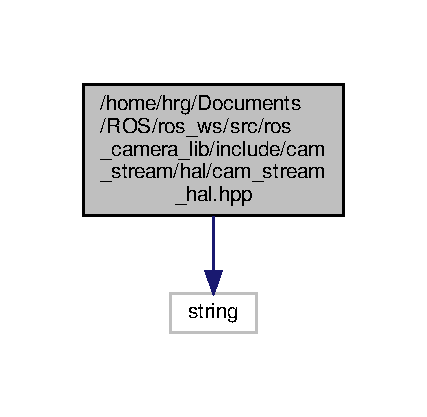
\includegraphics[width=205pt]{cam__stream__hal_8hpp__incl}
\end{center}
\end{figure}
This graph shows which files directly or indirectly include this file\+:\nopagebreak
\begin{figure}[H]
\begin{center}
\leavevmode
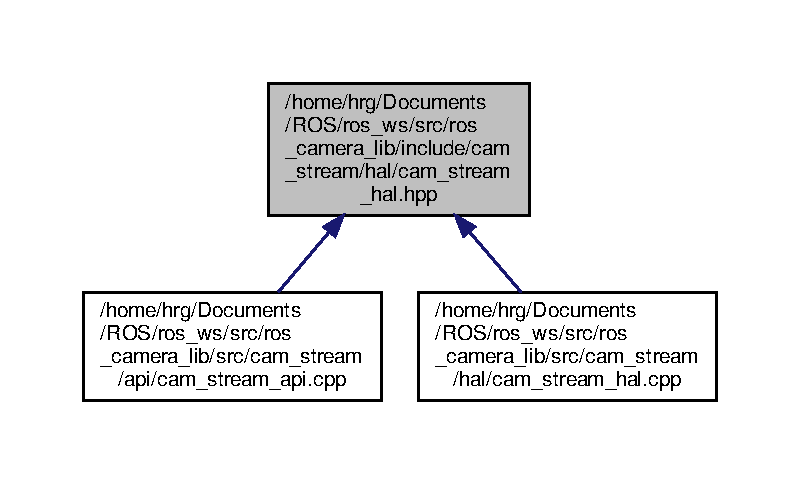
\includegraphics[width=350pt]{cam__stream__hal_8hpp__dep__incl}
\end{center}
\end{figure}
\subsection*{Functions}
\begin{DoxyCompactItemize}
\item 
void \hyperlink{cam__stream__hal_8hpp_a1e11c2994e4c097b343c3c92bb3a0e76}{hal\+\_\+init} (int argc, char $\ast$$\ast$argv, std\+::string node\+\_\+name, int video\+\_\+source)
\item 
int \hyperlink{cam__stream__hal_8hpp_a320d4712f522fc5d60f9469e8b173210}{hal\+\_\+ok} (void)
\item 
void \hyperlink{cam__stream__hal_8hpp_a8c47344dc199b3ce95ae4342b6ba91bf}{publish\+\_\+img} (void)
\item 
void \hyperlink{cam__stream__hal_8hpp_adbab9ad5f150267e43a88b8c6ae35b88}{finish\+\_\+hal} (void)
\end{DoxyCompactItemize}


\subsection{Function Documentation}
\mbox{\Hypertarget{cam__stream__hal_8hpp_adbab9ad5f150267e43a88b8c6ae35b88}\label{cam__stream__hal_8hpp_adbab9ad5f150267e43a88b8c6ae35b88}} 
\index{cam\+\_\+stream\+\_\+hal.\+hpp@{cam\+\_\+stream\+\_\+hal.\+hpp}!finish\+\_\+hal@{finish\+\_\+hal}}
\index{finish\+\_\+hal@{finish\+\_\+hal}!cam\+\_\+stream\+\_\+hal.\+hpp@{cam\+\_\+stream\+\_\+hal.\+hpp}}
\subsubsection{\texorpdfstring{finish\+\_\+hal()}{finish\_hal()}}
{\footnotesize\ttfamily void finish\+\_\+hal (\begin{DoxyParamCaption}\item[{void}]{ }\end{DoxyParamCaption})}

Release resources. \mbox{\Hypertarget{cam__stream__hal_8hpp_a1e11c2994e4c097b343c3c92bb3a0e76}\label{cam__stream__hal_8hpp_a1e11c2994e4c097b343c3c92bb3a0e76}} 
\index{cam\+\_\+stream\+\_\+hal.\+hpp@{cam\+\_\+stream\+\_\+hal.\+hpp}!hal\+\_\+init@{hal\+\_\+init}}
\index{hal\+\_\+init@{hal\+\_\+init}!cam\+\_\+stream\+\_\+hal.\+hpp@{cam\+\_\+stream\+\_\+hal.\+hpp}}
\subsubsection{\texorpdfstring{hal\+\_\+init()}{hal\_init()}}
{\footnotesize\ttfamily void hal\+\_\+init (\begin{DoxyParamCaption}\item[{int}]{argc,  }\item[{char $\ast$$\ast$}]{argv,  }\item[{std\+::string}]{node\+\_\+name,  }\item[{int}]{video\+\_\+source }\end{DoxyParamCaption})}

Initialize necessary variables and R\+OS environment. 
\begin{DoxyParams}{Parameters}
{\em argc} & Number of arguments referred to ros\+::init, in case they exist. \\
\hline
{\em argv} & Value of arguments referred to ros\+::init, in case they exist. \\
\hline
{\em node\+\_\+name} & Name of the publisher. \\
\hline
{\em video\+\_\+source} & Identifier of the camera to use. \\
\hline
\end{DoxyParams}
\mbox{\Hypertarget{cam__stream__hal_8hpp_a320d4712f522fc5d60f9469e8b173210}\label{cam__stream__hal_8hpp_a320d4712f522fc5d60f9469e8b173210}} 
\index{cam\+\_\+stream\+\_\+hal.\+hpp@{cam\+\_\+stream\+\_\+hal.\+hpp}!hal\+\_\+ok@{hal\+\_\+ok}}
\index{hal\+\_\+ok@{hal\+\_\+ok}!cam\+\_\+stream\+\_\+hal.\+hpp@{cam\+\_\+stream\+\_\+hal.\+hpp}}
\subsubsection{\texorpdfstring{hal\+\_\+ok()}{hal\_ok()}}
{\footnotesize\ttfamily int hal\+\_\+ok (\begin{DoxyParamCaption}\item[{void}]{ }\end{DoxyParamCaption})}

Function that checks for the correct running of the system. \mbox{\Hypertarget{cam__stream__hal_8hpp_a8c47344dc199b3ce95ae4342b6ba91bf}\label{cam__stream__hal_8hpp_a8c47344dc199b3ce95ae4342b6ba91bf}} 
\index{cam\+\_\+stream\+\_\+hal.\+hpp@{cam\+\_\+stream\+\_\+hal.\+hpp}!publish\+\_\+img@{publish\+\_\+img}}
\index{publish\+\_\+img@{publish\+\_\+img}!cam\+\_\+stream\+\_\+hal.\+hpp@{cam\+\_\+stream\+\_\+hal.\+hpp}}
\subsubsection{\texorpdfstring{publish\+\_\+img()}{publish\_img()}}
{\footnotesize\ttfamily void publish\+\_\+img (\begin{DoxyParamCaption}\item[{void}]{ }\end{DoxyParamCaption})}

Read image from source and publish it. 
\hypertarget{cam__stream__api_8cpp}{}\section{/home/hrg/\+Documents/\+R\+O\+S/ros\+\_\+ws/src/ros\+\_\+camera\+\_\+lib/src/cam\+\_\+stream/api/cam\+\_\+stream\+\_\+api.cpp File Reference}
\label{cam__stream__api_8cpp}\index{/home/hrg/\+Documents/\+R\+O\+S/ros\+\_\+ws/src/ros\+\_\+camera\+\_\+lib/src/cam\+\_\+stream/api/cam\+\_\+stream\+\_\+api.\+cpp@{/home/hrg/\+Documents/\+R\+O\+S/ros\+\_\+ws/src/ros\+\_\+camera\+\_\+lib/src/cam\+\_\+stream/api/cam\+\_\+stream\+\_\+api.\+cpp}}
{\ttfamily \#include \char`\"{}cam\+\_\+stream/api/cam\+\_\+stream\+\_\+api.\+hpp\char`\"{}}\newline
{\ttfamily \#include \char`\"{}cam\+\_\+stream/hal/cam\+\_\+stream\+\_\+hal.\+hpp\char`\"{}}\newline
Include dependency graph for cam\+\_\+stream\+\_\+api.\+cpp\+:\nopagebreak
\begin{figure}[H]
\begin{center}
\leavevmode
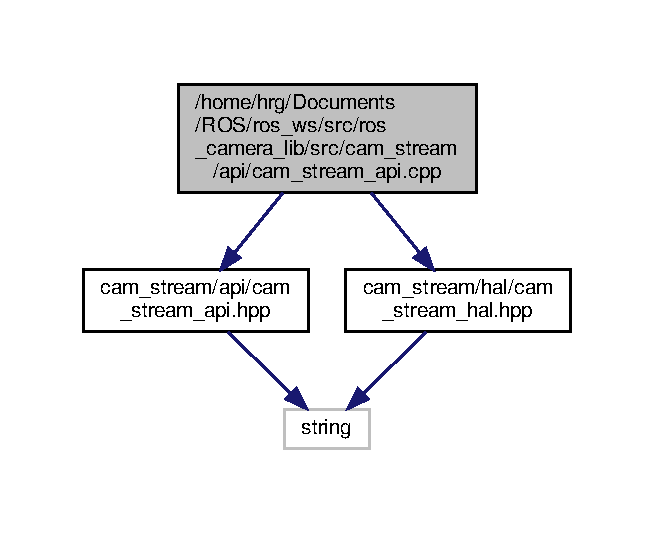
\includegraphics[width=314pt]{cam__stream__api_8cpp__incl}
\end{center}
\end{figure}
\subsection*{Functions}
\begin{DoxyCompactItemize}
\item 
void \hyperlink{cam__stream__api_8cpp_a071b3460290577ea5f2dde4bbceb43a3}{system\+\_\+init} (int argc, char $\ast$$\ast$argv, std\+::string node\+\_\+name, int video\+\_\+source)
\item 
int \hyperlink{cam__stream__api_8cpp_a77353b4935e897316414f01ccd30b117}{system\+\_\+ok} (void)
\item 
void \hyperlink{cam__stream__api_8cpp_aa1f1f7d9c7b32ebc5ee26f4d9748d99f}{stream} (void)
\item 
void \hyperlink{cam__stream__api_8cpp_ac6d72bbe9a798feae197f4c8ce164b08}{finish\+\_\+system} (void)
\end{DoxyCompactItemize}


\subsection{Function Documentation}
\mbox{\Hypertarget{cam__stream__api_8cpp_ac6d72bbe9a798feae197f4c8ce164b08}\label{cam__stream__api_8cpp_ac6d72bbe9a798feae197f4c8ce164b08}} 
\index{cam\+\_\+stream\+\_\+api.\+cpp@{cam\+\_\+stream\+\_\+api.\+cpp}!finish\+\_\+system@{finish\+\_\+system}}
\index{finish\+\_\+system@{finish\+\_\+system}!cam\+\_\+stream\+\_\+api.\+cpp@{cam\+\_\+stream\+\_\+api.\+cpp}}
\subsubsection{\texorpdfstring{finish\+\_\+system()}{finish\_system()}}
{\footnotesize\ttfamily void finish\+\_\+system (\begin{DoxyParamCaption}\item[{void}]{ }\end{DoxyParamCaption})}

Function in charge of releasing the system resources. \mbox{\Hypertarget{cam__stream__api_8cpp_aa1f1f7d9c7b32ebc5ee26f4d9748d99f}\label{cam__stream__api_8cpp_aa1f1f7d9c7b32ebc5ee26f4d9748d99f}} 
\index{cam\+\_\+stream\+\_\+api.\+cpp@{cam\+\_\+stream\+\_\+api.\+cpp}!stream@{stream}}
\index{stream@{stream}!cam\+\_\+stream\+\_\+api.\+cpp@{cam\+\_\+stream\+\_\+api.\+cpp}}
\subsubsection{\texorpdfstring{stream()}{stream()}}
{\footnotesize\ttfamily void stream (\begin{DoxyParamCaption}\item[{void}]{ }\end{DoxyParamCaption})}

Function in charge of streaming the image. \mbox{\Hypertarget{cam__stream__api_8cpp_a071b3460290577ea5f2dde4bbceb43a3}\label{cam__stream__api_8cpp_a071b3460290577ea5f2dde4bbceb43a3}} 
\index{cam\+\_\+stream\+\_\+api.\+cpp@{cam\+\_\+stream\+\_\+api.\+cpp}!system\+\_\+init@{system\+\_\+init}}
\index{system\+\_\+init@{system\+\_\+init}!cam\+\_\+stream\+\_\+api.\+cpp@{cam\+\_\+stream\+\_\+api.\+cpp}}
\subsubsection{\texorpdfstring{system\+\_\+init()}{system\_init()}}
{\footnotesize\ttfamily void system\+\_\+init (\begin{DoxyParamCaption}\item[{int}]{argc,  }\item[{char $\ast$$\ast$}]{argv,  }\item[{std\+::string}]{node\+\_\+name,  }\item[{int}]{video\+\_\+source }\end{DoxyParamCaption})}

Initialize necessary variables and R\+OS environment. 
\begin{DoxyParams}{Parameters}
{\em argc} & Number of arguments, in case they exist. \\
\hline
{\em argv} & Value of arguments, in case they exist. \\
\hline
{\em node\+\_\+name} & Name of the publisher. \\
\hline
{\em video\+\_\+source} & Identifier of the camera to use. \\
\hline
\end{DoxyParams}
\mbox{\Hypertarget{cam__stream__api_8cpp_a77353b4935e897316414f01ccd30b117}\label{cam__stream__api_8cpp_a77353b4935e897316414f01ccd30b117}} 
\index{cam\+\_\+stream\+\_\+api.\+cpp@{cam\+\_\+stream\+\_\+api.\+cpp}!system\+\_\+ok@{system\+\_\+ok}}
\index{system\+\_\+ok@{system\+\_\+ok}!cam\+\_\+stream\+\_\+api.\+cpp@{cam\+\_\+stream\+\_\+api.\+cpp}}
\subsubsection{\texorpdfstring{system\+\_\+ok()}{system\_ok()}}
{\footnotesize\ttfamily int system\+\_\+ok (\begin{DoxyParamCaption}\item[{void}]{ }\end{DoxyParamCaption})}

Function that checks for the correct running of the system. 
\hypertarget{cam__stream_8cpp}{}\section{/home/hrg/\+Documents/\+R\+O\+S/ros\+\_\+ws/src/ros\+\_\+camera\+\_\+lib/src/cam\+\_\+stream/app/cam\+\_\+stream.cpp File Reference}
\label{cam__stream_8cpp}\index{/home/hrg/\+Documents/\+R\+O\+S/ros\+\_\+ws/src/ros\+\_\+camera\+\_\+lib/src/cam\+\_\+stream/app/cam\+\_\+stream.\+cpp@{/home/hrg/\+Documents/\+R\+O\+S/ros\+\_\+ws/src/ros\+\_\+camera\+\_\+lib/src/cam\+\_\+stream/app/cam\+\_\+stream.\+cpp}}
{\ttfamily \#include \char`\"{}cam\+\_\+stream/api/cam\+\_\+stream\+\_\+api.\+hpp\char`\"{}}\newline
Include dependency graph for cam\+\_\+stream.\+cpp\+:\nopagebreak
\begin{figure}[H]
\begin{center}
\leavevmode
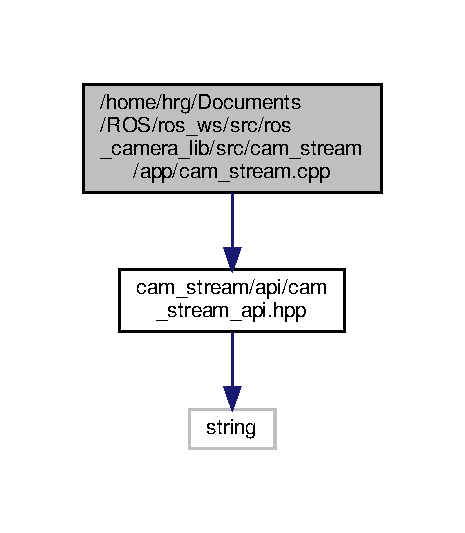
\includegraphics[width=223pt]{cam__stream_8cpp__incl}
\end{center}
\end{figure}
\subsection*{Macros}
\begin{DoxyCompactItemize}
\item 
\mbox{\Hypertarget{cam__stream_8cpp_a8cc8d559acdd2f74085b20977182d5b7}\label{cam__stream_8cpp_a8cc8d559acdd2f74085b20977182d5b7}} 
\#define {\bfseries N\+O\+D\+E\+\_\+\+N\+A\+ME}~\char`\"{}cam\+\_\+stream\char`\"{}
\item 
\mbox{\Hypertarget{cam__stream_8cpp_a3f86f6649dced75f11414cf68e6ac6ad}\label{cam__stream_8cpp_a3f86f6649dced75f11414cf68e6ac6ad}} 
\#define {\bfseries C\+A\+M\+\_\+\+ID}~0
\end{DoxyCompactItemize}
\subsection*{Functions}
\begin{DoxyCompactItemize}
\item 
int \hyperlink{cam__stream_8cpp_a3c04138a5bfe5d72780bb7e82a18e627}{main} (int argc, char $\ast$$\ast$argv)
\end{DoxyCompactItemize}


\subsection{Function Documentation}
\mbox{\Hypertarget{cam__stream_8cpp_a3c04138a5bfe5d72780bb7e82a18e627}\label{cam__stream_8cpp_a3c04138a5bfe5d72780bb7e82a18e627}} 
\index{cam\+\_\+stream.\+cpp@{cam\+\_\+stream.\+cpp}!main@{main}}
\index{main@{main}!cam\+\_\+stream.\+cpp@{cam\+\_\+stream.\+cpp}}
\subsubsection{\texorpdfstring{main()}{main()}}
{\footnotesize\ttfamily int main (\begin{DoxyParamCaption}\item[{int}]{argc,  }\item[{char $\ast$$\ast$}]{argv }\end{DoxyParamCaption})}

Main logic. 
\begin{DoxyParams}{Parameters}
{\em argc} & Number of arguments received. \\
\hline
{\em argv} & Value of arguments received. \\
\hline
\end{DoxyParams}
\begin{DoxySeeAlso}{See also}
\hyperlink{cam__stream__api_8cpp_a071b3460290577ea5f2dde4bbceb43a3}{system\+\_\+init()} 

\hyperlink{cam__stream__api_8cpp_a77353b4935e897316414f01ccd30b117}{system\+\_\+ok()} 

\hyperlink{cam__stream__api_8cpp_aa1f1f7d9c7b32ebc5ee26f4d9748d99f}{stream()} 

\hyperlink{cam__stream__api_8cpp_ac6d72bbe9a798feae197f4c8ce164b08}{finish\+\_\+system()} 
\end{DoxySeeAlso}

\hypertarget{cam__stream__hal_8cpp}{}\section{/home/hrg/\+Documents/\+R\+O\+S/ros\+\_\+ws/src/ros\+\_\+camera\+\_\+lib/src/cam\+\_\+stream/hal/cam\+\_\+stream\+\_\+hal.cpp File Reference}
\label{cam__stream__hal_8cpp}\index{/home/hrg/\+Documents/\+R\+O\+S/ros\+\_\+ws/src/ros\+\_\+camera\+\_\+lib/src/cam\+\_\+stream/hal/cam\+\_\+stream\+\_\+hal.\+cpp@{/home/hrg/\+Documents/\+R\+O\+S/ros\+\_\+ws/src/ros\+\_\+camera\+\_\+lib/src/cam\+\_\+stream/hal/cam\+\_\+stream\+\_\+hal.\+cpp}}
{\ttfamily \#include \char`\"{}cam\+\_\+stream/hal/cam\+\_\+stream\+\_\+hal.\+hpp\char`\"{}}\newline
{\ttfamily \#include $<$stdio.\+h$>$}\newline
{\ttfamily \#include \char`\"{}ros/ros.\+h\char`\"{}}\newline
{\ttfamily \#include \char`\"{}cv\+\_\+bridge/cv\+\_\+bridge.\+h\char`\"{}}\newline
{\ttfamily \#include \char`\"{}sensor\+\_\+msgs/\+Image.\+h\char`\"{}}\newline
{\ttfamily \#include \char`\"{}sensor\+\_\+msgs/image\+\_\+encodings.\+h\char`\"{}}\newline
{\ttfamily \#include \char`\"{}image\+\_\+transport/image\+\_\+transport.\+h\char`\"{}}\newline
{\ttfamily \#include \char`\"{}opencv2/highgui.\+hpp\char`\"{}}\newline
{\ttfamily \#include \char`\"{}opencv2/core.\+hpp\char`\"{}}\newline
{\ttfamily \#include \char`\"{}opencv2/imgproc.\+hpp\char`\"{}}\newline
Include dependency graph for cam\+\_\+stream\+\_\+hal.\+cpp\+:\nopagebreak
\begin{figure}[H]
\begin{center}
\leavevmode
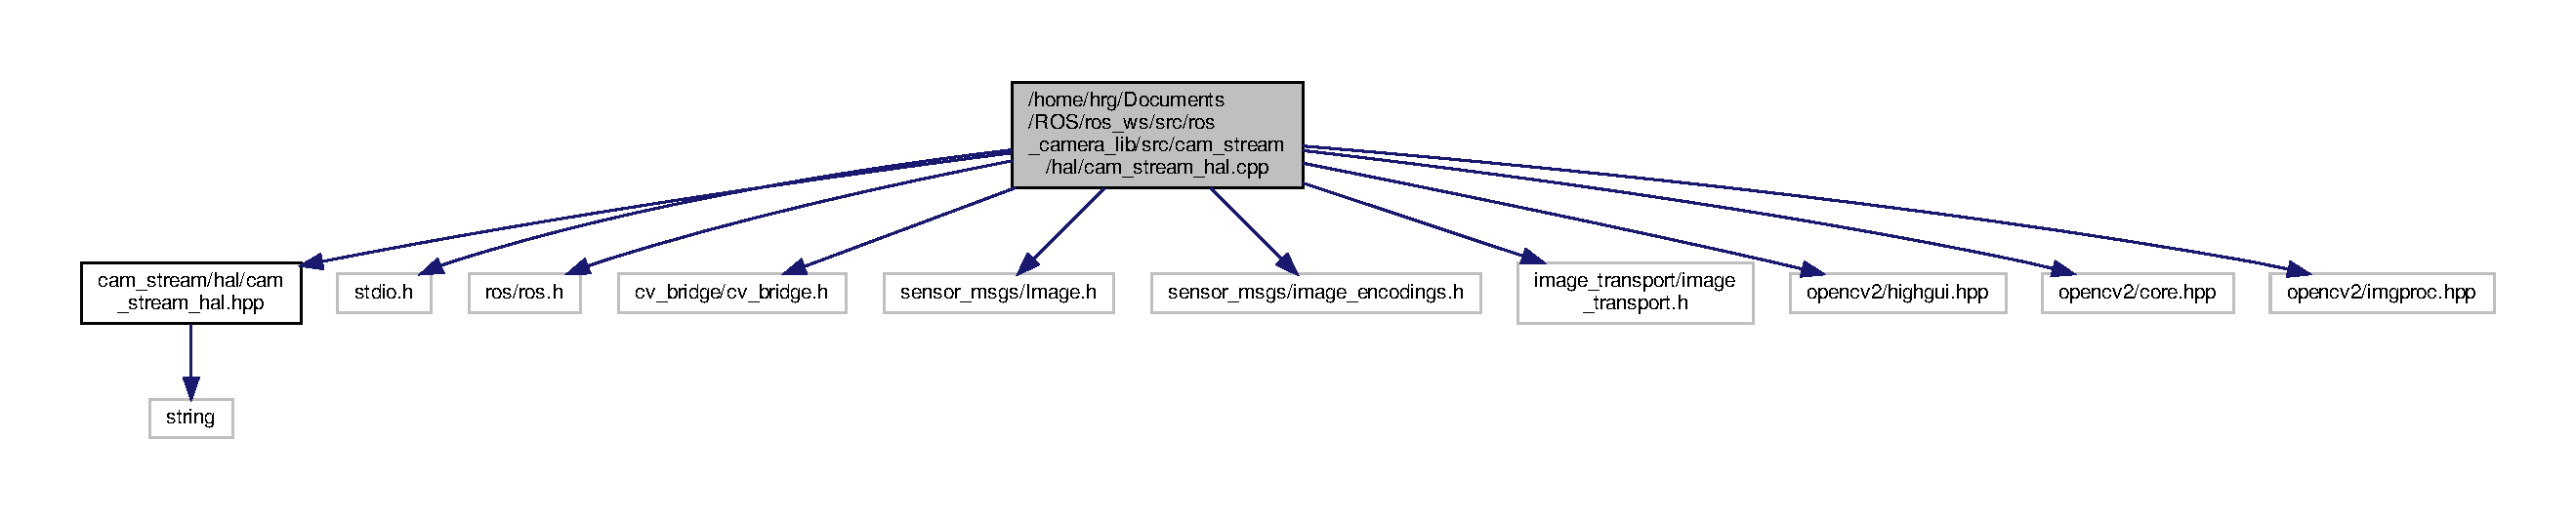
\includegraphics[width=350pt]{cam__stream__hal_8cpp__incl}
\end{center}
\end{figure}
\subsection*{Macros}
\begin{DoxyCompactItemize}
\item 
\mbox{\Hypertarget{cam__stream__hal_8cpp_ab3e92c6de76c27d00095b01f9445576d}\label{cam__stream__hal_8cpp_ab3e92c6de76c27d00095b01f9445576d}} 
\#define {\bfseries R\+O\+S\+\_\+\+L\+O\+O\+P\+\_\+\+R\+A\+TE}~3
\end{DoxyCompactItemize}
\subsection*{Functions}
\begin{DoxyCompactItemize}
\item 
void \hyperlink{cam__stream__hal_8cpp_a1e11c2994e4c097b343c3c92bb3a0e76}{hal\+\_\+init} (int argc, char $\ast$$\ast$argv, std\+::string node\+\_\+name, int video\+\_\+source)
\item 
int \hyperlink{cam__stream__hal_8cpp_a320d4712f522fc5d60f9469e8b173210}{hal\+\_\+ok} (void)
\item 
void \hyperlink{cam__stream__hal_8cpp_a8c47344dc199b3ce95ae4342b6ba91bf}{publish\+\_\+img} (void)
\item 
void \hyperlink{cam__stream__hal_8cpp_adbab9ad5f150267e43a88b8c6ae35b88}{finish\+\_\+hal} (void)
\end{DoxyCompactItemize}


\subsection{Function Documentation}
\mbox{\Hypertarget{cam__stream__hal_8cpp_adbab9ad5f150267e43a88b8c6ae35b88}\label{cam__stream__hal_8cpp_adbab9ad5f150267e43a88b8c6ae35b88}} 
\index{cam\+\_\+stream\+\_\+hal.\+cpp@{cam\+\_\+stream\+\_\+hal.\+cpp}!finish\+\_\+hal@{finish\+\_\+hal}}
\index{finish\+\_\+hal@{finish\+\_\+hal}!cam\+\_\+stream\+\_\+hal.\+cpp@{cam\+\_\+stream\+\_\+hal.\+cpp}}
\subsubsection{\texorpdfstring{finish\+\_\+hal()}{finish\_hal()}}
{\footnotesize\ttfamily void finish\+\_\+hal (\begin{DoxyParamCaption}\item[{void}]{ }\end{DoxyParamCaption})}

Release resources. \mbox{\Hypertarget{cam__stream__hal_8cpp_a1e11c2994e4c097b343c3c92bb3a0e76}\label{cam__stream__hal_8cpp_a1e11c2994e4c097b343c3c92bb3a0e76}} 
\index{cam\+\_\+stream\+\_\+hal.\+cpp@{cam\+\_\+stream\+\_\+hal.\+cpp}!hal\+\_\+init@{hal\+\_\+init}}
\index{hal\+\_\+init@{hal\+\_\+init}!cam\+\_\+stream\+\_\+hal.\+cpp@{cam\+\_\+stream\+\_\+hal.\+cpp}}
\subsubsection{\texorpdfstring{hal\+\_\+init()}{hal\_init()}}
{\footnotesize\ttfamily void hal\+\_\+init (\begin{DoxyParamCaption}\item[{int}]{argc,  }\item[{char $\ast$$\ast$}]{argv,  }\item[{std\+::string}]{node\+\_\+name,  }\item[{int}]{video\+\_\+source }\end{DoxyParamCaption})}

Initialize necessary variables and R\+OS environment. 
\begin{DoxyParams}{Parameters}
{\em argc} & Number of arguments referred to ros\+::init, in case they exist. \\
\hline
{\em argv} & Value of arguments referred to ros\+::init, in case they exist. \\
\hline
{\em node\+\_\+name} & Name of the publisher. \\
\hline
{\em video\+\_\+source} & Identifier of the camera to use. \\
\hline
\end{DoxyParams}
\mbox{\Hypertarget{cam__stream__hal_8cpp_a320d4712f522fc5d60f9469e8b173210}\label{cam__stream__hal_8cpp_a320d4712f522fc5d60f9469e8b173210}} 
\index{cam\+\_\+stream\+\_\+hal.\+cpp@{cam\+\_\+stream\+\_\+hal.\+cpp}!hal\+\_\+ok@{hal\+\_\+ok}}
\index{hal\+\_\+ok@{hal\+\_\+ok}!cam\+\_\+stream\+\_\+hal.\+cpp@{cam\+\_\+stream\+\_\+hal.\+cpp}}
\subsubsection{\texorpdfstring{hal\+\_\+ok()}{hal\_ok()}}
{\footnotesize\ttfamily int hal\+\_\+ok (\begin{DoxyParamCaption}\item[{void}]{ }\end{DoxyParamCaption})}

Function that checks for the correct running of the system. \mbox{\Hypertarget{cam__stream__hal_8cpp_a8c47344dc199b3ce95ae4342b6ba91bf}\label{cam__stream__hal_8cpp_a8c47344dc199b3ce95ae4342b6ba91bf}} 
\index{cam\+\_\+stream\+\_\+hal.\+cpp@{cam\+\_\+stream\+\_\+hal.\+cpp}!publish\+\_\+img@{publish\+\_\+img}}
\index{publish\+\_\+img@{publish\+\_\+img}!cam\+\_\+stream\+\_\+hal.\+cpp@{cam\+\_\+stream\+\_\+hal.\+cpp}}
\subsubsection{\texorpdfstring{publish\+\_\+img()}{publish\_img()}}
{\footnotesize\ttfamily void publish\+\_\+img (\begin{DoxyParamCaption}\item[{void}]{ }\end{DoxyParamCaption})}

Read image from source and publish it. 
%--- End generated contents ---

% Index
\backmatter
\newpage
\phantomsection
\clearemptydoublepage
\addcontentsline{toc}{chapter}{Index}
\printindex

\end{document}
